\chapter{Results and Discussion}
\label{chp:Results and Discussion}
This chapter documents the results from the trial conducted on the Ear-Monitor. The aim is to quantify the level of comparability between the Ear-Monitor's and benchmark device's measurements and through this get an understanding of the level of accuracy of the Ear-Monitor's measurements. Comparative analysis is done on each of the medical signs measurements made by the Ear-Monitor by comparing its measurements to those made by selected benchmark devices. Each participant is acting as his/her own control is this type of analysis. Results are discussed one at a time in this chapter.

\section{Temperature Results}
During each recording session, 15 Ear-Monitor data points and 3 ET 100-A benchmark data points are collected. It is assumed that the participant's core temperature stays constant during the duration of the recording session. Therefor the average ET 100-A benchmark measurement and the average Ear-Monitor measurement are compared. 2 participants' data was removed due to faulty recording sessions.

\medskip

The Ear-Monitor data points are analysed in terms of correlation with the ET 100-A benchmark measurements, intra session variation and the absolute mean errors. Results from the two calibration approaches are discussed separately.

\subsection{Calibration group results}
Equation \ref{eq:TempCal} is used to calculate tympanic temperature for all participants. Figure \ref{fig:Temp1Scatter} shows a scatterplot of the average Ear-Monitor vs. ET 100-A data points for the 28 recording sessions with temperature measurements.

\begin{figure}[H]
   \centering
   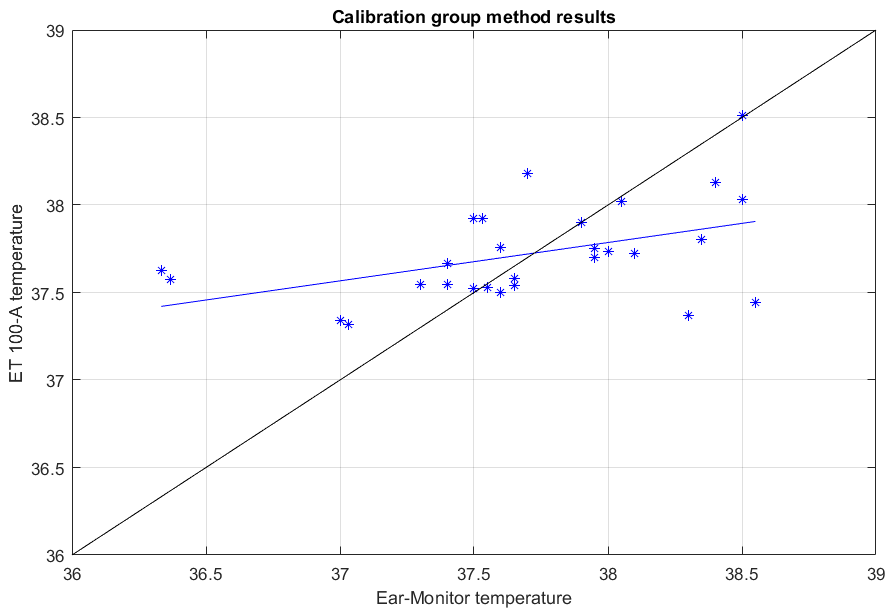
\includegraphics[width=12cm,height=7.5cm]{figs/Temp1Scatter.png}
   \caption{---}
   \label{fig:Temp1Scatter}
\end{figure}

The results for each session are summirised in Table \ref{tab:ResultsTemp}.

\subsection{Intra-participant calibration results}
This method used the data from the first recording session to calibrate the Ear-Monitor, and the data from the second session is used to evaluate this method. Figure \ref{fig:Temp2Scatter} shows a scatterplot of the average Ear-Monitor vs. ET 100-A data points for the 14 second recording sessions.

\begin{figure}[H]
   \centering
   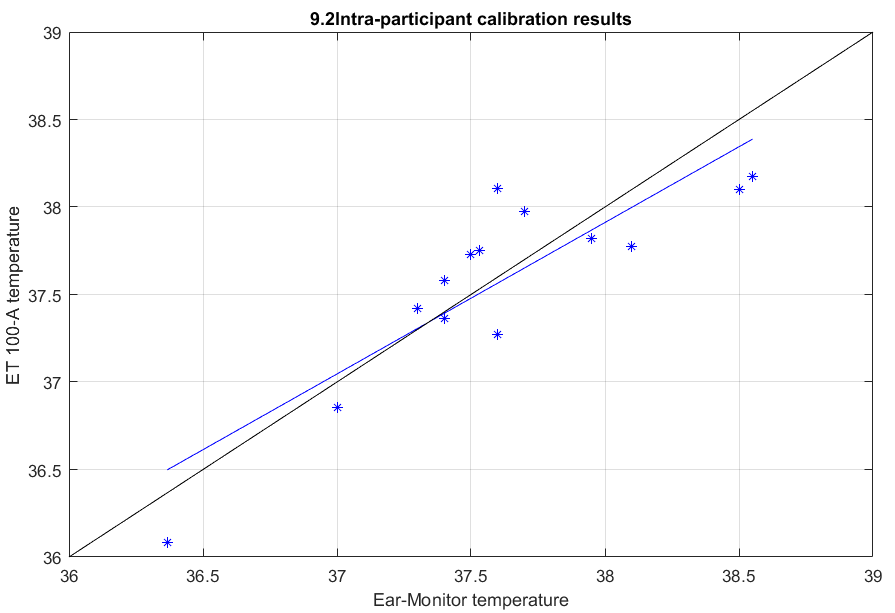
\includegraphics[width=12cm,height=7.5cm]{figs/Temp2Scatter.png}
   \caption{---}
   \label{fig:Temp2Scatter}
\end{figure}

\subsection{Temperature results discussion}
Blablabla...


\section{Heart Rate Results}
The Ear-Monitor uses an IR PPG obtained for the ear canal to detect pulse peaks via a beat detection algorithm. The average period between 10 successive detected beats are used to calculate the heart rate. The beat detection algorithm is at the core of the heart rate functionality of the Ear-Monitor, and therefore it is be evaluated independently. This is followed by comparative analysis between the individual beat periods and 10-beat moving average heart rates of the Ear-Monitor and Nexus-10 physiological monitor.

\subsection{Beat Detection Algorithm Evaluation Results}
The beat detection algorithm used by the Ear-Monitor is first tested on open source data from PhysioNet.org, and then on the data collected during the trial. These results of these two tests are discussed separately. 

\subsubsection{PhysioNet Data Test}
The beat detection algorithm is PPG data from the open-source MIMIC Database on PhysioNet.org \citep{PhysioNet}. This data was recorded from patients in intensive care units and is made available for developing and testing intelligent monitoring systems. PPG data is recorded with clinical finger pulse oximeters.

\medskip

Ten minute segments of 14 different patients are used to test the algorithm. Each set of data also includes an ECG signal, which is used to identify the benchmark beats. Table \ref{tab:PhysioNet} summarises the results from this test.

\begin{table}[H]
\caption{Results of the beat detection algorithm on the PhysioNet data}
\label{tab:PhysioNet}
\centering
\begin{tabular}{|P{3cm}| P{3cm}| P{3cm} |P{3cm}|} 
\hline
Record No.	&	Actual No. Beats	&	False Positives	&	False negatives\\ 
\hline
039		&	1337				&	0				&	0\\
\hline
041		& 	1030				&	1				&	7\\
\hline
055		&	1021				&	0				&	0\\
\hline
211		&	891					&	2				&	8\\
\hline
212		&	845					&	0				&	15\\
\hline
216		&	763					&	0				&	1\\
\hline
218		&	697					&	0				&	1\\
\hline
219		&	720					&	0				&	0\\
\hline
221		&	776					&	0				&	4\\
\hline
224		&	863					&	0				&	0\\
\hline
230		&	871					&	7				&	36\\
\hline
237		&	777					&	2				&	17\\
\hline
240		&	816					&	1				&	2\\
\hline	
252		&	594					&	0				&	0\\
\hline
\end{tabular}
\end{table}

Of the 12001 beats in all the test data, 13 (0.108\%) false positives were detected and 91 (0.758\%) false negatives. Even though the beat-detection algorithm was designed and tuned using PPGs collected form the ear canal wall, it can accurately detect beats from finger pulse oximeters. This results demonstrates the robustness of the algorithm. Most false detections occurred where signals were corrupted by noise. It also illustrate how the SSF can extract beats, even from a noisy signal by including a plot of the PPG and subsequent SSF plus detected beats.

\subsubsection{Trial Data Test}
Next the algorithm is tested using the data collected during the trial. The number of beats detected by the Ear-Monitor will be compared to the actual number of heartbeats. The Nexus-10's supporting software, BioTrace+, has a peak detection algorithm, but it was found that is misses some peaks. To ensure accurate benchmark peak detection, the PPG from the Nexus-10 is inspected manually and peaks are marked by a human annotator. Figure \ref{BeatDetectionTest} shows plots of (a) the Ear-Monitor SSF with detected beats and (b) the Nexus-10 PPG signal with annotated beats. In this example 100\% of the peaks are detected by Ear-Monitor.

\begin{figure}[H]
   \centering
   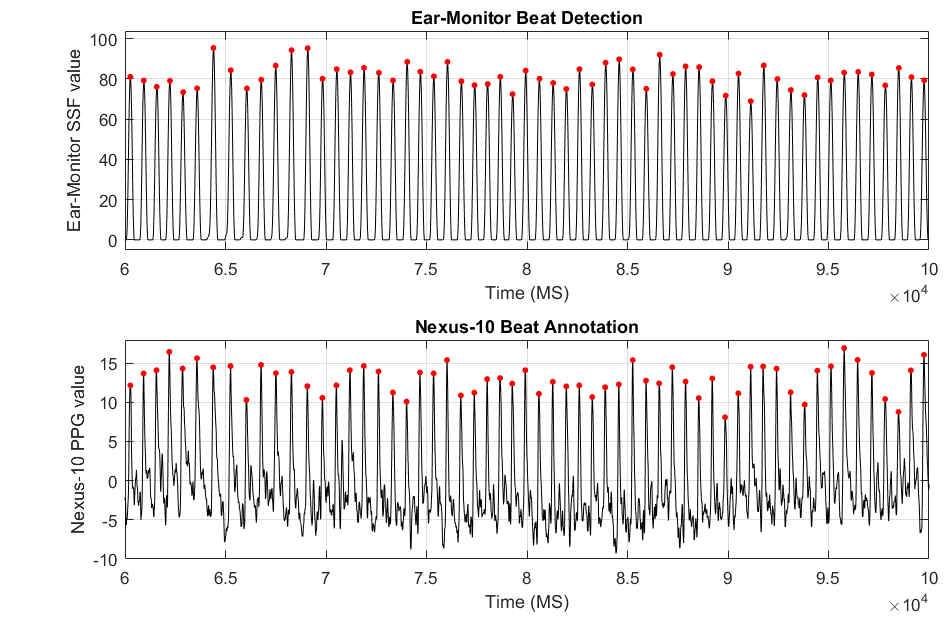
\includegraphics[width=12cm,height=7.5cm]{figs/BeatDetectionTest.png}
   \caption{Plots of (a) the Ear-Monitor SSF with detected beats and (b) the Nexus-10 PPG signal with annotated beats} %Marga1_Data
   \label{fig:BeatDetectionTest}
\end{figure}

Table \ref{tab:BeatDetectionTest} summarises the results to the beat detection evaluation.

\begin{table}[H]
\caption{Results of the beat detection algorithm on the PhysioNet data}
\label{tab:BeatDetectionTest}
\centering
\begin{tabular}{|P{1.9cm}| P{1.9cm}| P{1.9cm} | P{1.9cm} | P{1.9cm} | P{1.9cm} |} 
\hline
Participant No.	&	 No. Nexus-10 Beats	&	No. Ear-Monitor Beats	&	False Positives & False Negatives & \%\\ 
\hline
1a	&	150	&	150	&	0	&	0	&	100	\\
\hline
1b	&	148	&	148	&	0	&	0	&	100	\\
\hline
2a	&	116	&	108	&	2	&	10	&	93.1	\\
\hline
2b	&	116	&	106	&	1	&	11	&	91.4	\\
\hline
3a	&	136	&	136	&	0	&	0	&	100	\\
\hline
3b	&	138	&	138	&	0	&	0	&	100	\\
\hline
4a	&	132	&	132	&	0	&	0	&	100	\\
\hline
4b	&	133	&	132	&	0	&	1	&	99.2	\\
\hline
5a	&	181	&	181	&	0	&	0	&	100	\\
\hline
5b	&	188	&	187	&	0	&	1	&	99.5	\\
\hline
6a	&	120	&	120	&	0	&	0	&	100	\\
\hline
6b	&	127	&	127	&	0	&	0	&	100	\\
\hline
7b	&	144	&	144	&	0	&	0	&	100	\\
\hline
7c	&	140	&	140	&	0	&	0	&	100	\\
\hline
8a	&	163	&	163	&	0	&	0	&	100	\\
\hline
8b	&	164	&	163	&	0	&	1	&	99.4	\\
\hline
9a	&	149	&	149	&	0	&	0	&	100	\\
\hline
9b	&	146	&	142	&	0	&	4	&	97.3	\\
\hline
10a	&	146	&	146	&	0	&	0	&	100	\\
\hline
10c	&	146	&	146	&	0	&	0	&	100	\\
\hline
11a	&	131	&	131	&	0	&	0	&	100	\\
\hline
11b	&	131	&	131	&	0	&	0	&	100	\\
\hline
12a	&	144	&	144	&	0	&	0	&	100	\\
\hline
12b	&	137	&	137	&	0	&	0	&	100	\\
\hline
13a	&	169	&	163	&	0	&	6	&	96.45	\\
\hline
13b	&	169	&	162	&	0	&	7	&	95.86	\\
\hline
14a	&	168	&	168	&	0	&	0	&	100	\\
\hline
14b	&	170	&	170	&	0	&	0	&	100	\\
\hline
15a	&	149	&	149	&	0	&	0	&	100	\\
\hline
15c	&	149	&	149	&	0	&	0	&	100	\\
\hline
16a	&	154	&	151	&	1	&	4	&	98.05	\\
\hline
16b	&	159	&	152	&	6	&	13	&	95.6	\\

\hline
\end{tabular}
\end{table}

Of the 4713 beats in all the participant trail data, 4655 (98.77\%) are successfully detected. 10 (0.21\%) false positives and 58 (1.23\%) false negatives are detected. It should also be noted the 51 of the false negatives are from the data collected from three of the participants.

Figure \ref{fig:BeatDetectionScatter} shows a scatted plot of the number of annotated Nexus-10 beats vs. the number of detected Ear-Monitor beats. Data recording sessions from all 16 trial participants are used, meaning 32 sets of data points are compared.

\begin{figure}[H]
   \centering
   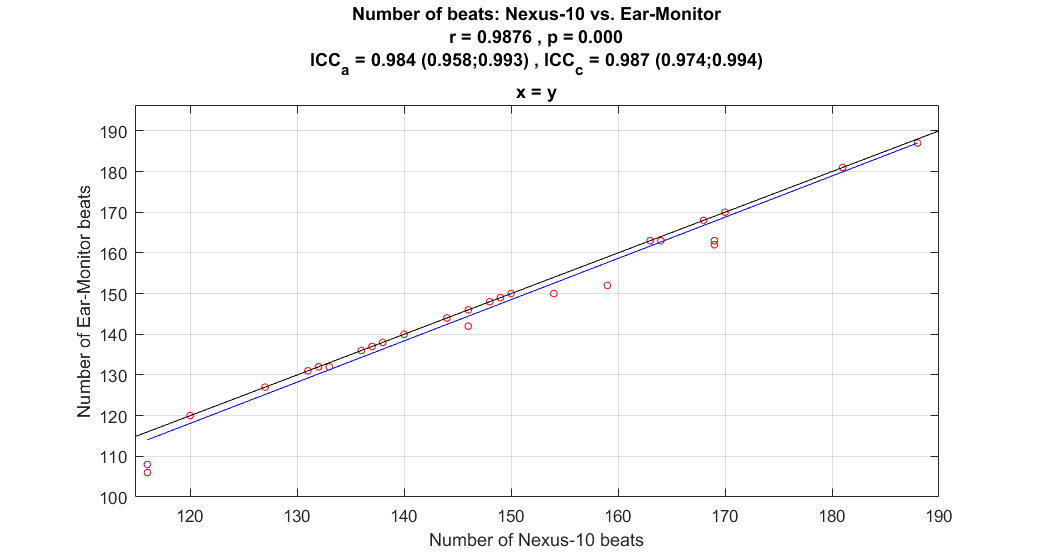
\includegraphics[width=12cm,height=7.5cm]{figs/BeatDetectionScatter.png}
   \caption{Number of beats: Nexus-10 vs. Ear-Monitor}
   \label{fig:BeatDetectionScatter}
\end{figure}

This test shows that the Ear-Monitor preforms well in its task of detection beats. The number of false negatives detected for the trial data is higher than for the PhysioNet data. This can be ascribed to the fact that the PPG from three of the participants was of a notably lower quality. Although the adaptive threshold method detected the majority if the peaks, the amplitude of the SSF peaks varied prominently and very low amplitudes were missed by the algorithm. This can be caused by low blood profusion in the ear canal or bad contact between the MAX30100 and the canal wall. This is a patient specific inaccuracy and can be overcome by an more customised ear probe. 

\subsection{Beat Period and Average Heart Rate Results}
The accuracy of the heat beat period is tested to see if beats and detected at the right position in time. The individual period between beats detected be the Ear-Monitor is compared to the period between beats annotated on the Nexus-10 PPG. Figure \ref{fig:PeriodScatter} shows a scatter plot of the Nexus-10 period vs. theEar-Monitor period. A total of 4569 periods are compared from all 16 participants.

\begin{figure}[H]
   \centering
   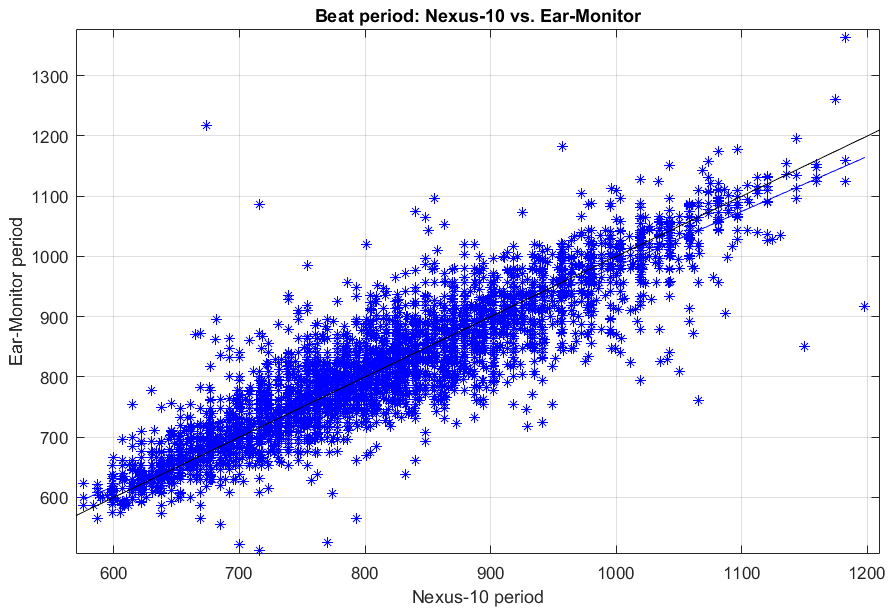
\includegraphics[width=12cm,height=7.5cm]{figs/PeriodScatter.png}
   \caption{Beat period: Nexus-10 vs. Ear-Monitor}
   \label{fig:PeriodScatter}
\end{figure}

The 10-beat average heart rate is calculate form the Ear-Monitor and Nexus-10 data and compared in the same way as with he beat periodes. Figure \ref{fig:HeartRateScatter} shows a scatter plot of the Nexus-10 heart rate vs. the Ear-Monitor heart rate. A total of 4258 periods are compared from all 16 participants.

\begin{figure}[H]
   \centering
   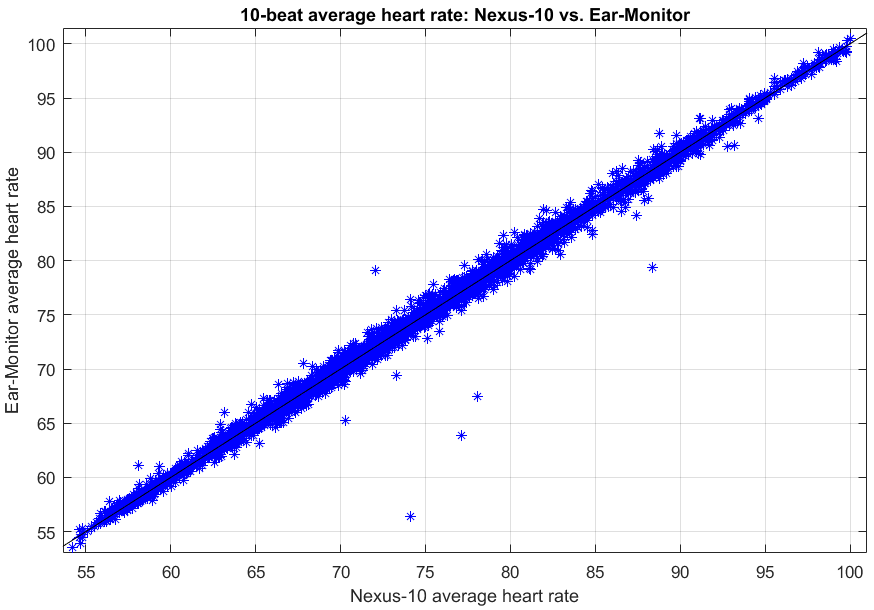
\includegraphics[width=12cm,height=7.5cm]{figs/HeartRateScatter.png}
   \caption{10-beat average heart rate: Nexus-10 vs. Ear-Monitor}
   \label{fig:HeartRateScatter}
\end{figure}

\subsection{Heart Rate Results Discussion}
Blablabla...
